\paragraph*{}
  Il est désormais temps d'implémenter notre LBM, l'algorithme ce décompose en trois étapes :
  \begin{itemize} \label{eq:defmeso}
    \itemb Initialisation :\\
    \emph{On définie les valeurs aux bornes et l'on applique les rebond sur les objets (on échange les populations).}
    \itemb Flux :\\
    \emph{On déplace les populations de $\ei \dt$.}
    \itemb Collision :\\
    \emph{On applique l'opérateur collision sur les populations $f_i$.}  
  \end{itemize}
  On répète ces étapes en boucle pour simuler le comportement du fluide.
  
  \begin{figure}[hbtp]
    \centering
    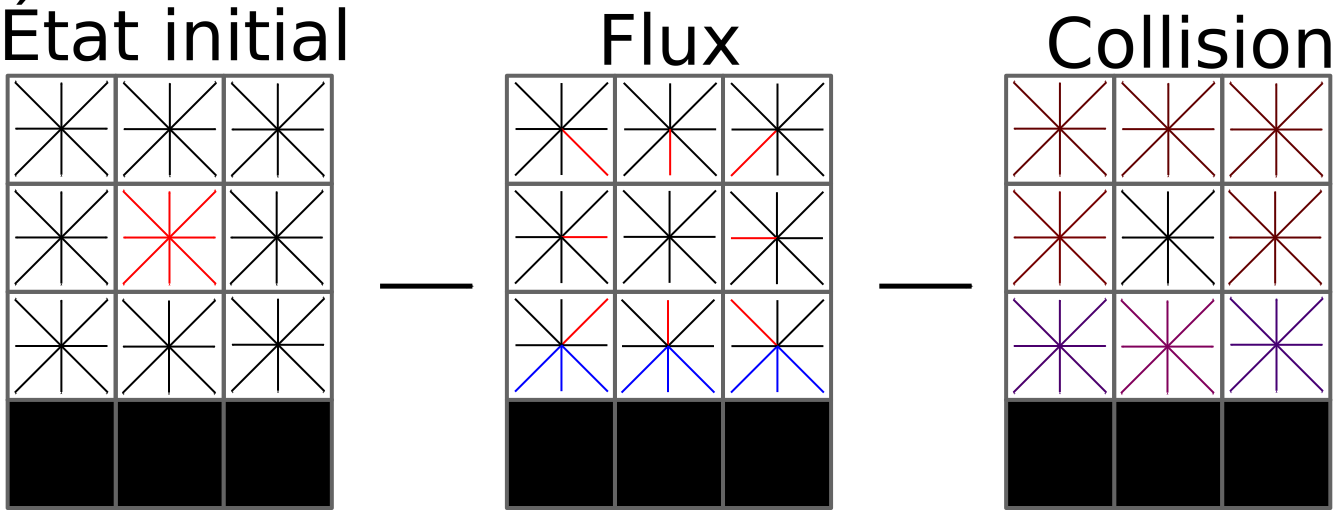
\includegraphics[width=\linewidth]{Fig/algorithme.pdf}
    \caption{Shéma des différentes étapes de résulotion de la LBM.}
  \end{figure}
  
   Cette structure est effectivement bien visible dans notre code {\sc Fortran}:
  \begin{minted}{fortran}
!===============================================================================
!                               The main program.
!===============================================================================
Program LBM2D
  Use Var
  Use Dconst, Only: L, H, N
  Implicit None
  Integer(4) :: dN, d = 100, ni = 0
  Call Allocatall             ! Alloue les variables en mémoire
  Call InitF                  ! Initialise les variables
  
  Do dN = 0, N
    If (Modulo(dN, d) == 0) Then      
      Call Savefile(ni)      ! Sauvegarde les valeurs intermédiaires pour pouvoir faire des animations
      ni = ni + 1
    End If

    CALL IOlet                ! Initialisation
    CALL Bound                ! Initialisation
    CALL Stream               ! Flux
    CALL CMacro               ! Collision : calcul les valeurs macro
    CALL CFeq                 ! Collision : calcul les valeurs de feq
    CALL Collide              ! Collision : applique l'opérateur collision
  End Do
  
  Call Deallocatall           ! Libère la mémoire
End Program LBM2D
  \end{minted}
  
  durant l'implémentation nous avons fait le choix d'utiliser des subroutines afin de minimiser l'impact mémoire (La 
  gestion de la mémoire est un problème critique dans notre code nous avons donc privilégié le passage par référence 
  plutôt que le passage par valeur).
  De plus pour accélérer notre code nous avons utilisée énormément de boucles Do en respectant l'ordre des indices,
  comme par exemple dans la subroutine collide :
  \begin{minted}{fortran}
!===============================================================================
!                             Collide Step
!===============================================================================
Subroutine Collide
  Use Var, Only: F, Feq
  Use Cconst, Only: itau, mitau
  Use Dconst, Only: L, H
  Use Lconst, Only: Q
  Implicit None
  Integer(4) :: i, j
  Integer(1) :: k
  
  Do j = 1, H
    Do i = 1, L
      Do k = 1, Q
        F(k,i,j)= mitau*F(k,i,j) + itau*Feq(k,i,j)
      End Do
    End Do
  End Do
End Subroutine
  \end{minted}
    cette subroutine est l'implémentation de l'équation \ref{eq:LBGK}.
  
  